% !TeX program = xelatex
% 保持 assets/blocks.pdf 与本文件的相对位置。用 XeLaTeX 连续编译两次。
% 题面和解答以可选中文字的 PDF 题块嵌入。
\documentclass[UTF8,a4paper,11pt]{ctexart}
\usepackage[left=21mm,right=21mm,top=20mm,bottom=18mm,headheight=24pt,headsep=6mm,footskip=10mm]{geometry}
\usepackage{graphicx,booktabs,tabularx,fancyhdr,needspace,xcolor}
\usepackage[unicode,bookmarksopen,bookmarksopenlevel=1,hidelinks]{hyperref}

\hypersetup{
  pdftitle={408 计算机网络历年真题},
  pdfsubject={2009—2026 年 408 计算机网络真题与参考答案}
}
\definecolor{ink}{HTML}{19232D}
\definecolor{muted}{HTML}{465568}
\definecolor{rulegray}{HTML}{C7CFD8}
\color{ink}

\setlength{\parindent}{0pt}
\setlength{\parskip}{0pt}
\raggedbottom
\pagestyle{fancy}
\fancyhf{}
\fancyhead[L]{\small\color{muted}408 计算机网络}
\fancyhead[R]{\small\color{muted}\nouppercase{\rightmark}}
\fancyfoot[C]{\small\color{muted}\thepage}
\renewcommand{\headrule}{\hbox to\headwidth{\color{rulegray}\leaders\hrule height .4pt\hfill}}
\ctexset{
  section = {format=\Large\bfseries\color{ink},beforeskip=13pt,afterskip=6pt},
  subsection = {format=\normalsize\bfseries\color{ink},beforeskip=9pt,afterskip=3pt}
}

\newcommand{\BlockWidth}{\linewidth}
\newcommand{\PlaceBlock}[3]{%
  \par\nointerlineskip
  \hbox to \linewidth{\hss
    \includegraphics[page=#1,#2,width=\BlockWidth,height=.92\textheight,keepaspectratio]{assets/blocks.pdf}%
  \hss}%
  \penalty#3\vskip2pt
}
\newcommand{\PaperBlock}[1]{\PlaceBlock{#1}{}{0}}
% 在完整小问或整图的边界保留分页点。参数依次为素材页、上裁切量、下裁切量、分页惩罚。
\newcommand{\PaperSlice}[4]{\PlaceBlock{#1}{trim=0 #3bp 0 #2bp,clip}{#4}}
\newcommand{\PartHeading}[3]{%
  \Needspace{#3bp}%
  \section*{#2}\label{#1}%
  \markboth{#2}{#2}%
  \addcontentsline{toc}{section}{#2}%
}
\newcommand{\YearHeading}[4]{%
  \Needspace{#3bp}%
  \subsection*{#2 年\hfill{\normalfont\small\color{muted}#4}}%
  \label{#1:#2}\addcontentsline{toc}{subsection}{#2 年}%
}
\newcommand{\AnswerYear}[1]{\hypertarget{answer-#1}{#1}}
\newcommand{\PageJump}[1]{\hyperref[#1]{\pageref*{#1}}}
\newcommand{\IndexYear}[1]{#1 & \PageJump{choice:#1} & \PageJump{big:#1}}

\begin{document}
\thispagestyle{plain}
{\LARGE\bfseries 408 计算机网络历年真题\par}
\vskip4pt
{\small\color{muted}2009—2026 年 · 144 道单选 · 19 道综合及交叉题\par}
\vskip9pt

\begingroup
\small
\renewcommand{\arraystretch}{1.10}
\begin{tabular*}{\linewidth}{@{\extracolsep{\fill}}rccrccrcc@{}}
\toprule
年份 & 单选页 & 综合页 & 年份 & 单选页 & 综合页 & 年份 & 单选页 & 综合页 \\
\midrule
\IndexYear{2009} & \IndexYear{2015} & \IndexYear{2021} \\
\IndexYear{2010} & \IndexYear{2016} & \IndexYear{2022} \\
\IndexYear{2011} & \IndexYear{2017} & \IndexYear{2023} \\
\IndexYear{2012} & \IndexYear{2018} & \IndexYear{2024} \\
\IndexYear{2013} & \IndexYear{2019} & \IndexYear{2025} \\
\IndexYear{2014} & \IndexYear{2020} & \IndexYear{2026} \\
\bottomrule
\end{tabular*}
\endgroup
\vskip6pt
{\small
\hyperref[choice-answer]{单选参考答案（第 \pageref*{choice-answer} 页）}
\quad
\hyperref[big-answer]{综合题参考解答（第 \pageref*{big-answer} 页）}\par}
\vskip5pt
{\small\color{muted}
2014 年第 42 题随第 43 题收录。2016 年综合题为第 41 题。2026 年采用公开回忆整理版。
试题与解答来自\href{https://eze-root.github.io/408/assignments/}{公开排版试题册与答案册}，2020 年第 35 题拓扑图取自\href{https://pgcode.cn/exams/408/years/2020/preview}{PGCode 题面}。\par}

\PartHeading{choice}{单项选择题}{126}
\YearHeading{choice}{2009}{91}{\hyperlink{answer-2009}{看单选答案}}
% 2009 年第 33 题，原 PDF 第 5 页，题块 1
\PaperBlock{1}
% 2009 年第 34 题，原 PDF 第 5 页，题块 1
\PaperBlock{2}
% 2009 年第 35 题，原 PDF 第 6 页，题块 1
\PaperBlock{3}
% 2009 年第 36 题，原 PDF 第 6 页，题块 1
\PaperBlock{4}
% 2009 年第 37 题，原 PDF 第 6 页，题块 1
\PaperBlock{5}
% 2009 年第 38 题，原 PDF 第 6 页，题块 1
\PaperBlock{6}
% 2009 年第 39 题，原 PDF 第 6 页，题块 1
\PaperBlock{7}
% 2009 年第 40 题，原 PDF 第 6 页，题块 1
\PaperBlock{8}
\YearHeading{choice}{2010}{91}{\hyperlink{answer-2010}{看单选答案}}
% 2010 年第 33 题，原 PDF 第 6 页，题块 1
\PaperBlock{10}
% 2010 年第 34 题，原 PDF 第 6 页，题块 1
\PaperBlock{11}
% 2010 年第 35 题，原 PDF 第 7 页，题块 1
\PaperBlock{12}
% 2010 年第 36 题，原 PDF 第 7 页，题块 1
\PaperBlock{13}
% 2010 年第 37 题，原 PDF 第 7 页，题块 1
\PaperBlock{14}
% 2010 年第 38 题，原 PDF 第 7 页，题块 1
\PaperBlock{15}
% 2010 年第 39 题，原 PDF 第 7 页，题块 1
\PaperBlock{16}
% 2010 年第 40 题，原 PDF 第 7 页，题块 1
\PaperBlock{17}
\YearHeading{choice}{2011}{91}{\hyperlink{answer-2011}{看单选答案}}
% 2011 年第 33 题，原 PDF 第 6 页，题块 1
\PaperBlock{19}
% 2011 年第 34 题，原 PDF 第 6 页，题块 1
\PaperBlock{20}
% 2011 年第 35 题，原 PDF 第 6 页，题块 1
\PaperBlock{21}
% 2011 年第 36 题，原 PDF 第 6 页，题块 1
\PaperBlock{22}
% 2011 年第 37 题，原 PDF 第 6 页，题块 1
\PaperBlock{23}
% 2011 年第 38 题，原 PDF 第 7 页，题块 1
\PaperBlock{24}
% 2011 年第 39 题，原 PDF 第 7 页，题块 1
\PaperBlock{25}
% 2011 年第 40 题，原 PDF 第 7 页，题块 1
\PaperBlock{26}
\YearHeading{choice}{2012}{91}{\hyperlink{answer-2012}{看单选答案}}
% 2012 年第 33 题，原 PDF 第 6 页，题块 1
\PaperBlock{28}
% 2012 年第 34 题，原 PDF 第 6 页，题块 1
\PaperBlock{29}
% 2012 年第 35 题，原 PDF 第 6 页，题块 1
\PaperBlock{30}
% 2012 年第 36 题，原 PDF 第 6 页，题块 1
\PaperBlock{31}
% 2012 年第 37 题，原 PDF 第 6 页，题块 1
\PaperBlock{32}
% 2012 年第 38 题，原 PDF 第 7 页，题块 1
\PaperBlock{33}
% 2012 年第 39 题，原 PDF 第 7 页，题块 1
\PaperBlock{34}
% 2012 年第 40 题，原 PDF 第 7 页，题块 1
\PaperBlock{35}
\YearHeading{choice}{2013}{91}{\hyperlink{answer-2013}{看单选答案}}
% 2013 年第 33 题，原 PDF 第 6 页，题块 1
\PaperBlock{37}
% 2013 年第 34 题，原 PDF 第 6 页，题块 1
\PaperBlock{38}
% 2013 年第 35 题，原 PDF 第 7 页，题块 1
\PaperBlock{39}
% 2013 年第 36 题，原 PDF 第 7 页，题块 1
\PaperBlock{40}
% 2013 年第 37 题，原 PDF 第 7 页，题块 1
\PaperBlock{41}
% 2013 年第 38 题，原 PDF 第 7 页，题块 1
\PaperBlock{42}
% 2013 年第 39 题，原 PDF 第 7 页，题块 1
\PaperBlock{43}
% 2013 年第 40 题，原 PDF 第 7 页，题块 1
\PaperBlock{44}
\YearHeading{choice}{2014}{91}{\hyperlink{answer-2014}{看单选答案}}
% 2014 年第 33 题，原 PDF 第 5 页，题块 1
\PaperBlock{46}
% 2014 年第 34 题，原 PDF 第 6 页，题块 1
\PaperBlock{47}
% 2014 年第 35 题，原 PDF 第 6 页，题块 1
\PaperBlock{48}
% 2014 年第 36 题，原 PDF 第 6 页，题块 1
\PaperBlock{49}
% 2014 年第 37 题，原 PDF 第 6 页，题块 1
\PaperBlock{50}
% 2014 年第 38 题，原 PDF 第 7 页，题块 1
\PaperBlock{51}
% 2014 年第 39 题，原 PDF 第 7 页，题块 1
\PaperBlock{52}
% 2014 年第 40 题，原 PDF 第 7 页，题块 1
\PaperBlock{53}
\YearHeading{choice}{2015}{91}{\hyperlink{answer-2015}{看单选答案}}
% 2015 年第 33 题，原 PDF 第 5 页，题块 1
\PaperBlock{56}
% 2015 年第 34 题，原 PDF 第 6 页，题块 1
\PaperBlock{57}
% 2015 年第 35 题，原 PDF 第 6 页，题块 1
\PaperBlock{58}
% 2015 年第 36 题，原 PDF 第 6 页，题块 1
\PaperBlock{59}
% 2015 年第 37 题，原 PDF 第 6 页，题块 1
\PaperBlock{60}
% 2015 年第 38 题，原 PDF 第 7 页，题块 1
\PaperBlock{61}
% 2015 年第 39 题，原 PDF 第 7 页，题块 1
\PaperBlock{62}
% 2015 年第 40 题，原 PDF 第 7 页，题块 1
\PaperBlock{63}
\YearHeading{choice}{2016}{275}{\hyperlink{answer-2016}{看单选答案}}
% 2016 年第 33 题，原 PDF 第 7 页，题块 1
\PaperBlock{65}
% 2016 年第 34 题，原 PDF 第 7 页，题块 1
\PaperBlock{66}
% 2016 年第 35 题，原 PDF 第 7 页，题块 1
\PaperBlock{67}
% 2016 年第 36 题，原 PDF 第 7 页，题块 1
\PaperBlock{68}
% 2016 年第 37 题，原 PDF 第 8 页，题块 1
\PaperBlock{69}
% 2016 年第 38 题，原 PDF 第 8 页，题块 1
\PaperBlock{70}
% 2016 年第 39 题，原 PDF 第 8 页，题块 1
\PaperBlock{71}
% 2016 年第 40 题，原 PDF 第 8 页，题块 1
\PaperBlock{72}
\YearHeading{choice}{2017}{108}{\hyperlink{answer-2017}{看单选答案}}
% 2017 年第 33 题，原 PDF 第 6 页，题块 1
\PaperBlock{74}
% 2017 年第 34 题，原 PDF 第 6 页，题块 1
\PaperBlock{75}
% 2017 年第 35 题，原 PDF 第 6 页，题块 1
\PaperBlock{76}
% 2017 年第 36 题，原 PDF 第 6 页，题块 1
\PaperBlock{77}
% 2017 年第 37 题，原 PDF 第 7 页，题块 1
\PaperBlock{78}
% 2017 年第 38 题，原 PDF 第 7 页，题块 1
\PaperBlock{79}
% 2017 年第 39 题，原 PDF 第 7 页，题块 1
\PaperBlock{80}
% 2017 年第 40 题，原 PDF 第 7 页，题块 1
\PaperBlock{81}
\YearHeading{choice}{2018}{91}{\hyperlink{answer-2018}{看单选答案}}
% 2018 年第 33 题，原 PDF 第 6 页，题块 1
\PaperBlock{83}
% 2018 年第 34 题，原 PDF 第 6 页，题块 1
\PaperBlock{84}
% 2018 年第 35 题，原 PDF 第 6 页，题块 1
\PaperBlock{85}
% 2018 年第 36 题，原 PDF 第 6 页，题块 1
\PaperBlock{86}
% 2018 年第 37 题，原 PDF 第 7 页，题块 1
\PaperBlock{87}
% 2018 年第 38 题，原 PDF 第 7 页，题块 1
\PaperBlock{88}
% 2018 年第 39 题，原 PDF 第 7 页，题块 1
\PaperBlock{89}
% 2018 年第 40 题，原 PDF 第 7 页，题块 1
\PaperBlock{90}
\YearHeading{choice}{2019}{91}{\hyperlink{answer-2019}{看单选答案}}
% 2019 年第 33 题，原 PDF 第 6 页，题块 1
\PaperBlock{92}
% 2019 年第 34 题，原 PDF 第 6 页，题块 1
\PaperBlock{93}
% 2019 年第 35 题，原 PDF 第 6 页，题块 1
\PaperBlock{94}
% 2019 年第 36 题，原 PDF 第 6 页，题块 1
\PaperBlock{95}
% 2019 年第 37 题，原 PDF 第 6 页，题块 1
\PaperBlock{96}
% 2019 年第 38 题，原 PDF 第 7 页，题块 1
\PaperBlock{97}
% 2019 年第 39 题，原 PDF 第 7 页，题块 1
\PaperBlock{98}
% 2019 年第 40 题，原 PDF 第 7 页，题块 1
\PaperBlock{99}
\YearHeading{choice}{2020}{292}{\hyperlink{answer-2020}{看单选答案}}
% 2020 年第 33 题，原 PDF 第 7 页，题块 1
\PaperBlock{101}
% 2020 年第 34 题，原 PDF 第 7 页，题块 1
\PaperBlock{102}
% 2020 年第 35 题，原 PDF 第 7 页，题块 1，含补入的拓扑图
\PaperBlock{103}
% 2020 年第 36 题，原 PDF 第 7 页，题块 1
\PaperBlock{104}
% 2020 年第 37 题，原 PDF 第 8 页，题块 1
\PaperBlock{105}
% 2020 年第 38 题，原 PDF 第 8 页，题块 1
\PaperBlock{106}
% 2020 年第 39 题，原 PDF 第 8 页，题块 1
\PaperBlock{107}
% 2020 年第 40 题，原 PDF 第 9 页，题块 1
\PaperBlock{108}
\YearHeading{choice}{2021}{91}{\hyperlink{answer-2021}{看单选答案}}
% 2021 年第 33 题，原 PDF 第 6 页，题块 1
\PaperBlock{110}
% 2021 年第 34 题，原 PDF 第 6 页，题块 1
\PaperBlock{111}
% 2021 年第 35 题，原 PDF 第 6 页，题块 1
\PaperBlock{112}
% 2021 年第 36 题，原 PDF 第 6 页，题块 1
\PaperBlock{113}
% 2021 年第 37 题，原 PDF 第 7 页，题块 1
\PaperBlock{114}
% 2021 年第 38 题，原 PDF 第 7 页，题块 1
\PaperBlock{115}
% 2021 年第 39 题，原 PDF 第 7 页，题块 1
\PaperBlock{116}
% 2021 年第 40 题，原 PDF 第 7 页，题块 1
\PaperBlock{117}
\YearHeading{choice}{2022}{91}{\hyperlink{answer-2022}{看单选答案}}
% 2022 年第 33 题，原 PDF 第 6 页，题块 1
\PaperBlock{119}
% 2022 年第 34 题，原 PDF 第 6 页，题块 1
\PaperBlock{120}
% 2022 年第 35 题，原 PDF 第 6 页，题块 1
\PaperBlock{121}
% 2022 年第 36 题，原 PDF 第 7 页，题块 1
\PaperBlock{122}
% 2022 年第 37 题，原 PDF 第 7 页，题块 1
\PaperBlock{123}
% 2022 年第 38 题，原 PDF 第 7 页，题块 1
\PaperBlock{124}
% 2022 年第 39 题，原 PDF 第 7 页，题块 1
\PaperBlock{125}
% 2022 年第 40 题，原 PDF 第 7 页，题块 1
\PaperBlock{126}
\YearHeading{choice}{2023}{216}{\hyperlink{answer-2023}{看单选答案}}
% 2023 年第 33 题，原 PDF 第 6 页，题块 1
\PaperBlock{128}
% 2023 年第 34 题，原 PDF 第 6 页，题块 1
\PaperBlock{129}
% 2023 年第 35 题，原 PDF 第 6 页，题块 1
\PaperBlock{130}
% 2023 年第 36 题，原 PDF 第 6 页，题块 1
\PaperBlock{131}
% 2023 年第 37 题，原 PDF 第 6 页，题块 1
\PaperBlock{132}
% 2023 年第 38 题，原 PDF 第 7 页，题块 1
\PaperBlock{133}
% 2023 年第 39 题，原 PDF 第 7 页，题块 1
\PaperBlock{134}
% 2023 年第 40 题，原 PDF 第 7 页，题块 1
\PaperBlock{135}
\YearHeading{choice}{2024}{241}{\hyperlink{answer-2024}{看单选答案}}
% 2024 年第 33 题，原 PDF 第 6 页，题块 1
\PaperBlock{137}
% 2024 年第 34 题，原 PDF 第 6 页，题块 1
\PaperBlock{138}
% 2024 年第 35 题，原 PDF 第 6 页，题块 1
\PaperBlock{139}
% 2024 年第 36 题，原 PDF 第 6 页，题块 1
\PaperBlock{140}
% 2024 年第 37 题，原 PDF 第 7 页，题块 1
\PaperBlock{141}
% 2024 年第 38 题，原 PDF 第 7 页，题块 1
\PaperBlock{142}
% 2024 年第 39 题，原 PDF 第 7 页，题块 1
\PaperBlock{143}
% 2024 年第 40 题，原 PDF 第 7 页，题块 1
\PaperBlock{144}
\YearHeading{choice}{2025}{283}{\hyperlink{answer-2025}{看单选答案}}
% 2025 年第 33 题，原 PDF 第 6 页，题块 1
\PaperBlock{146}
% 2025 年第 34 题，原 PDF 第 6 页，题块 1
\PaperBlock{147}
% 2025 年第 35 题，原 PDF 第 6 页，题块 1
\PaperBlock{148}
% 2025 年第 36 题，原 PDF 第 6 页，题块 1
\PaperBlock{149}
% 2025 年第 37 题，原 PDF 第 7 页，题块 1
\PaperBlock{150}
% 2025 年第 38 题，原 PDF 第 7 页，题块 1
\PaperBlock{151}
% 2025 年第 39 题，原 PDF 第 7 页，题块 1
\PaperBlock{152}
% 2025 年第 40 题，原 PDF 第 7 页，题块 1
\PaperBlock{153}
\YearHeading{choice}{2026}{91}{\hyperlink{answer-2026}{看单选答案}}
% 2026 年第 33 题，原 PDF 第 6 页，题块 1
\PaperBlock{155}
% 2026 年第 34 题，原 PDF 第 6 页，题块 1
\PaperBlock{156}
% 2026 年第 35 题，原 PDF 第 7 页，题块 1
\PaperBlock{157}
% 2026 年第 36 题，原 PDF 第 7 页，题块 1
\PaperBlock{158}
% 2026 年第 37 题，原 PDF 第 8 页，题块 1
\PaperBlock{159}
% 2026 年第 38 题，原 PDF 第 9 页，题块 1
\PaperBlock{160}
% 2026 年第 39 题，原 PDF 第 9 页，题块 1
\PaperBlock{161}
% 2026 年第 40 题，原 PDF 第 9 页，题块 1
\PaperBlock{162}
\PartHeading{big}{综合应用题}{372}
\YearHeading{big}{2009}{342}{}
% 2009 年第 47 题，原 PDF 第 13 页，题块 1
\PaperSlice{9}{0.000}{103.660}{85}
\PaperSlice{9}{324.930}{-0.000}{0}
\YearHeading{big}{2010}{196}{}
% 2010 年第 47 题，原 PDF 第 14 页，题块 1
\PaperBlock{18}
\YearHeading{big}{2011}{266}{}
% 2011 年第 47 题，原 PDF 第 15 页，题块 1
\PaperSlice{27}{0.000}{274.212}{85}
\PaperSlice{27}{246.047}{171.804}{85}
\PaperSlice{27}{348.455}{-0.000}{0}
\YearHeading{big}{2012}{283}{}
% 2012 年第 47 题，原 PDF 第 14 页，题块 1
\PaperSlice{36}{0.000}{389.621}{85}
\PaperSlice{36}{264.019}{-0.000}{0}
\YearHeading{big}{2013}{290}{}
% 2013 年第 47 题，原 PDF 第 14 页，题块 1
\PaperSlice{45}{0.000}{127.315}{85}
\PaperSlice{45}{271.031}{-0.000}{0}
\YearHeading{big}{2014}{268}{}
% 2014 年第 42 题，原 PDF 第 9 页，题块 1
\begin{minipage}{\linewidth}
\PaperBlock{54}
\begingroup
\small
\setlength{\tabcolsep}{4pt}
\renewcommand{\arraystretch}{1.23}
\noindent\begin{tabularx}{\linewidth}{|l|l|c|c|c|c|>{\raggedright\arraybackslash}X|}
\hline
\multicolumn{2}{|c|}{} & $R_1$ 的 LSI & $R_2$ 的 LSI & $R_3$ 的 LSI & $R_4$ 的 LSI & 备注\\
\hline
\multicolumn{2}{|l|}{Router ID} & 10.1.1.1 & 10.1.1.2 & 10.1.1.5 & 10.1.1.6 & 标识路由器的 IP 地址\\
\hline
Link1 & ID & 10.1.1.2 & 10.1.1.1 & 10.1.1.6 & 10.1.1.5 & 所连路由器的 Router ID\\
& IP & 10.1.1.1 & 10.1.1.2 & 10.1.1.5 & 10.1.1.6 & Link1 的本地 IP 地址\\
& Metric & 3 & 3 & 6 & 6 & Link1 的费用\\
\hline
Link2 & ID & 10.1.1.5 & 10.1.1.6 & 10.1.1.1 & 10.1.1.2 & 所连路由器的 Router ID\\
& IP & 10.1.1.9 & 10.1.1.13 & 10.1.1.10 & 10.1.1.14 & Link2 的本地 IP 地址\\
& Metric & 2 & 4 & 2 & 4 & Link2 的费用\\
\hline
Net1 & Prefix & 192.1.1.0/24 & 192.1.6.0/24 & 192.1.5.0/24 & 192.1.7.0/24 & 直达网络 Net1 的网络前缀\\
& Metric & 1 & 1 & 1 & 1 & 到达直连网络 Net1 的费用\\
\hline
\end{tabularx}\par
\endgroup\end{minipage}\par\penalty90\vskip4pt
\PaperBlock{184}
% 2014 年第 43 题，原 PDF 第 10 页，题块 1
\PaperBlock{55}
\YearHeading{big}{2015}{314}{}
% 2015 年第 47 题，原 PDF 第 14 页，题块 1
\PaperSlice{64}{0.000}{171.960}{85}
\PaperSlice{64}{296.100}{86.912}{85}
\PaperSlice{64}{381.148}{-0.000}{0}
\YearHeading{big}{2016}{146}{共用\hyperref[choice:2016]{单选第 33 题的拓扑图}}
% 2016 年第 41 题，原 PDF 第 9 页，题块 1
\PaperSlice{73}{0.000}{121.048}{85}
\PaperSlice{73}{121.436}{0.000}{0}
\YearHeading{big}{2017}{392}{}
% 2017 年第 47 题，原 PDF 第 14 页，题块 1
\PaperSlice{82}{0.000}{120.408}{85}
\PaperSlice{82}{377.381}{-0.000}{0}
\YearHeading{big}{2018}{279}{}
% 2018 年第 47 题，原 PDF 第 14 页，题块 1
\PaperSlice{91}{0.000}{70.164}{85}
\PaperSlice{91}{259.490}{-0.000}{0}
\YearHeading{big}{2019}{350}{}
% 2019 年第 47 题，原 PDF 第 14 页，题块 1
\PaperSlice{100}{0.000}{103.020}{85}
\PaperSlice{100}{333.265}{0.000}{0}
\YearHeading{big}{2020}{345}{}
% 2020 年第 47 题，原 PDF 第 16 页，题块 1
\PaperSlice{109}{0.000}{86.912}{85}
\PaperSlice{109}{327.998}{0.000}{0}
\YearHeading{big}{2021}{408}{}
% 2021 年第 47 题，原 PDF 第 14 页，题块 1
\PaperSlice{118}{0.000}{86.272}{85}
\PaperSlice{118}{394.129}{-0.000}{0}
\YearHeading{big}{2022}{326}{}
% 2022 年第 47 题，原 PDF 第 14 页，题块 1
\PaperSlice{127}{0.000}{137.796}{85}
\PaperSlice{127}{308.491}{0.000}{0}
\YearHeading{big}{2023}{173}{}
% 2023 年第 47 题，原 PDF 第 14 页，题块 1
\PaperSlice{136}{0.000}{137.796}{85}
\PaperSlice{136}{150.367}{69.524}{85}
\PaperSlice{136}{218.639}{-0.000}{0}
\YearHeading{big}{2024}{318}{}
% 2024 年第 47 题，原 PDF 第 14 页，题块 1
\PaperSlice{145}{0.000}{276.686}{85}
\PaperSlice{145}{300.622}{156.890}{85}
\PaperSlice{145}{420.418}{0.000}{0}
\YearHeading{big}{2025}{259}{}
% 2025 年第 47 题，原 PDF 第 14 页，题块 1
\PaperSlice{154}{0.000}{191.880}{85}
\PaperSlice{154}{239.463}{122.328}{85}
\PaperSlice{154}{309.015}{0.000}{0}
\YearHeading{big}{2026}{232}{}
% 2026 年第 47 题，原 PDF 第 16 页，题块 1
\PaperSlice{163}{0.000}{404.639}{85}
\PaperSlice{163}{211.000}{137.796}{85}
\PaperSlice{163}{477.843}{69.524}{85}
\PaperSlice{163}{546.115}{0.000}{0}

\PartHeading{choice-answer}{单项选择题参考答案}{214}
\begingroup
\small
\setlength{\tabcolsep}{3.8pt}
\renewcommand{\arraystretch}{1.15}
\noindent\begin{tabular*}{\linewidth}{@{\extracolsep{\fill}}r*{8}{c}@{\hspace{1.4em}}r*{8}{c}@{}}
\toprule
年份 & 33 & 34 & 35 & 36 & 37 & 38 & 39 & 40 &
年份 & 33 & 34 & 35 & 36 & 37 & 38 & 39 & 40 \\
\midrule
\AnswerYear{2009} & B & B & C & A & D & D & C & A & \AnswerYear{2018} & B & C & D & D & D & C & B & D \\
\AnswerYear{2010} & C & C & D & C & B & D & A & A & \AnswerYear{2019} & C & A & B & B & B & C & D & B \\
\AnswerYear{2011} & A & B & B & D & D & C & C & B & \AnswerYear{2020} & C & B & C & D & A & D & C & D \\
\AnswerYear{2012} & B & C & A & B & C & A & D & D & \AnswerYear{2021} & B & A & B & B & D & B & D & C \\
\AnswerYear{2013} & B & A & D & B & A & B & B & A & \AnswerYear{2022} & B & C & B & D & B & C & D & B \\
\AnswerYear{2014} & C & B & D & C & B & A & B & D & \AnswerYear{2023} & D & C & B & C & D & A & B & D \\
\AnswerYear{2015} & D & A & B & B & A & C & A & C & \AnswerYear{2024} & B & C & D & B & D & D & C & D \\
\AnswerYear{2016} & C & C & D & B & B & D & C & C & \AnswerYear{2025} & B & C & C & C & B & A & B & A \\
\AnswerYear{2017} & A & D & B & A & D & C & A & C & \AnswerYear{2026} & B & D & B & B & B & A & C & D \\
\bottomrule
\end{tabular*}\par
\endgroup

\PartHeading{big-answer}{综合题参考解答}{223}
\renewcommand{\BlockWidth}{.95\linewidth}
\Needspace{201bp}
\subsection*{2009 年第 47 题}
% 2009 年第 47 题解答，原 PDF 第 14 页，题块 1
\PaperSlice{164}{0.000}{297.918}{85}
\PaperSlice{164}{191.232}{0.000}{0}
\Needspace{146bp}
\subsection*{2010 年第 47 题}
% 2010 年第 47 题解答，原 PDF 第 13 页，题块 1
\PaperSlice{165}{0.000}{99.632}{85}
\PaperSlice{165}{129.880}{0.000}{0}
\Needspace{92bp}
\subsection*{2011 年第 47 题}
% 2011 年第 47 题解答，原 PDF 第 13 页，题块 1
\PaperSlice{166}{0.000}{138.128}{85}
\PaperSlice{166}{71.996}{73.244}{85}
\PaperSlice{166}{136.880}{0.000}{0}
\Needspace{189bp}
\subsection*{2012 年第 47 题}
% 2012 年第 47 题解答，原 PDF 第 13 页，题块 1
\PaperSlice{167}{0.000}{129.828}{85}
\PaperSlice{167}{178.016}{0.000}{0}
\Needspace{156bp}
\subsection*{2013 年第 47 题}
% 2013 年第 47 题解答，原 PDF 第 13 页，题块 1
\PaperSlice{168}{0.000}{92.992}{85}
\PaperSlice{168}{141.974}{0.000}{0}
\Needspace{76bp}
\subsection*{2014 年第 42 题}
% 2014 年第 42 题解答，原 PDF 第 9 页，题块 1
\PaperSlice{169}{0.000}{442.361}{85}
\PaperSlice{169}{54.608}{0.000}{0}
% 2014 年第 42 题解答，原 PDF 第 10 页，题块 2
\PaperSlice{170}{0.000}{107.092}{85}
\PaperSlice{170}{296.377}{0.000}{0}
\Needspace{183bp}
\subsection*{2014 年第 43 题}
% 2014 年第 43 题解答，原 PDF 第 11 页，题块 1
\PaperBlock{171}
\Needspace{109bp}
\subsection*{2015 年第 47 题}
% 2015 年第 47 题解答，原 PDF 第 13 页，题块 1
\PaperSlice{172}{0.000}{111.300}{85}
\PaperSlice{172}{89.384}{0.000}{0}
\Needspace{98bp}
\subsection*{2016 年第 41 题}
% 2016 年第 41 题解答，原 PDF 第 7 页，题块 1
\PaperSlice{173}{0.000}{213.540}{85}
\PaperSlice{173}{78.356}{148.656}{85}
\PaperSlice{173}{143.240}{-0.000}{0}
\Needspace{114bp}
\subsection*{2017 年第 47 题}
% 2017 年第 47 题解答，原 PDF 第 13 页，题块 1
\PaperSlice{174}{0.000}{229.260}{85}
\PaperSlice{174}{95.744}{164.376}{85}
\PaperSlice{174}{160.628}{99.492}{85}
\PaperSlice{174}{225.512}{0.000}{0}
\Needspace{188bp}
\subsection*{2018 年第 47 题}
% 2018 年第 47 题解答，原 PDF 第 13 页，题块 1
\PaperBlock{175}
\Needspace{181bp}
\subsection*{2019 年第 47 题}
% 2019 年第 47 题解答，原 PDF 第 13 页，题块 1
\PaperBlock{176}
\Needspace{200bp}
\subsection*{2020 年第 47 题}
% 2020 年第 47 题解答，原 PDF 第 13 页，题块 1
\PaperBlock{177}
\Needspace{76bp}
\subsection*{2021 年第 47 题}
% 2021 年第 47 题解答，原 PDF 第 13 页，题块 1
\PaperSlice{178}{0.000}{134.596}{85}
\PaperSlice{178}{54.608}{0.000}{0}
\Needspace{151bp}
\subsection*{2022 年第 47 题}
% 2022 年第 47 题解答，原 PDF 第 13 页，题块 1
\PaperBlock{179}
\Needspace{121bp}
\subsection*{2023 年第 47 题}
% 2023 年第 47 题解答，原 PDF 第 13 页，题块 1
\PaperSlice{180}{0.000}{170.872}{85}
\PaperSlice{180}{102.852}{-0.000}{0}
\Needspace{167bp}
\subsection*{2024 年第 47 题}
% 2024 年第 47 题解答，原 PDF 第 13 页，题块 1
\PaperBlock{181}
\Needspace{165bp}
\subsection*{2025 年第 47 题}
% 2025 年第 47 题解答，原 PDF 第 9 页，题块 1
\PaperSlice{182}{0.000}{247.474}{85}
\PaperSlice{182}{151.182}{118.574}{85}
\PaperSlice{182}{280.082}{-0.000}{0}
\Needspace{166bp}
\subsection*{2026 年第 47 题}
% 2026 年第 47 题解答，原 PDF 第 8 页，题块 1
\PaperBlock{183}
\end{document}
